\section{Proposed Method}
\label{sec:method}

\subsection{Overview}

The method has five layers. First, a multi-column DSP placement instance is decomposed into several single-column strip subproblems following the \rsad strategy. Second, we justify the use of the order-consistency (OC) condition from the HPWL viewpoint. Third, under OC, the weighted HPWL objective is converted into a shortest-path problem on a state DAG and solved exactly by dynamic programming. Fourth, when the strip is tall, a CTR-based reduction shrinks an $m \times h$ instance to an $h \times h$ core problem and then expands the solution back. Finally, an outer timing-driven loop updates net weights according to longest-wire violations and repeatedly invokes the exact strip solver.

\subsection{Multi-Column Decomposition}

Our exact solver is built for single-column strip placement, so a multi-column FPGA placement must first be decomposed into strip subproblems. Here we deliberately follow the \rsad strategy instead of introducing a new decomposition principle. Candidate column cuts are evaluated by estimating the wirelength range they can induce. The \rsad analytical wirelength formula provides a lower bound for a given cut pattern, while the row-sweep construction provides a corresponding upper bound. These bounds are used to estimate the attainable wirelength range of each strip type and to choose the most promising column partition.

After a column partition is fixed, each strip is treated as a single-column placement problem. The contribution of the present paper therefore begins after the decomposition step: the column partitioning remains \rsad-style, while the new technical content lies in the exact weighted strip solver and its timing-driven extension.

\subsection{Why the OC Condition Is Legitimate}

The first theoretical question is whether it is legitimate to restrict attention to the OC-structured solution space introduced by \rsad.

\textbf{Proposition 1.}
If a single-column placement is optimal under OC, then swapping any pair of DSP macros cannot decrease HPWL. Equivalently, an OC-optimal solution is locally optimal with respect to arbitrary two-swaps.

The proof sketch is direct and does not require a separate induction on swap distance. Consider an arbitrary two-swap between macros $a$ and $b$. If the swap preserves OC, then HPWL cannot decrease because the original solution is already optimal within the OC-feasible set. The nontrivial case is when the swap breaks OC. In that case, all relative layouts can be reduced to three basic positional patterns:
\begin{itemize}[leftmargin=*,topsep=2pt,itemsep=2pt]
\item the two macros lie on the same row or the same column,
\item the two macros lie on different rows and different columns, and
\item boundary or corner configurations, which are degenerate forms of the previous two patterns.
\end{itemize}

\begin{figure}[t]
\centering
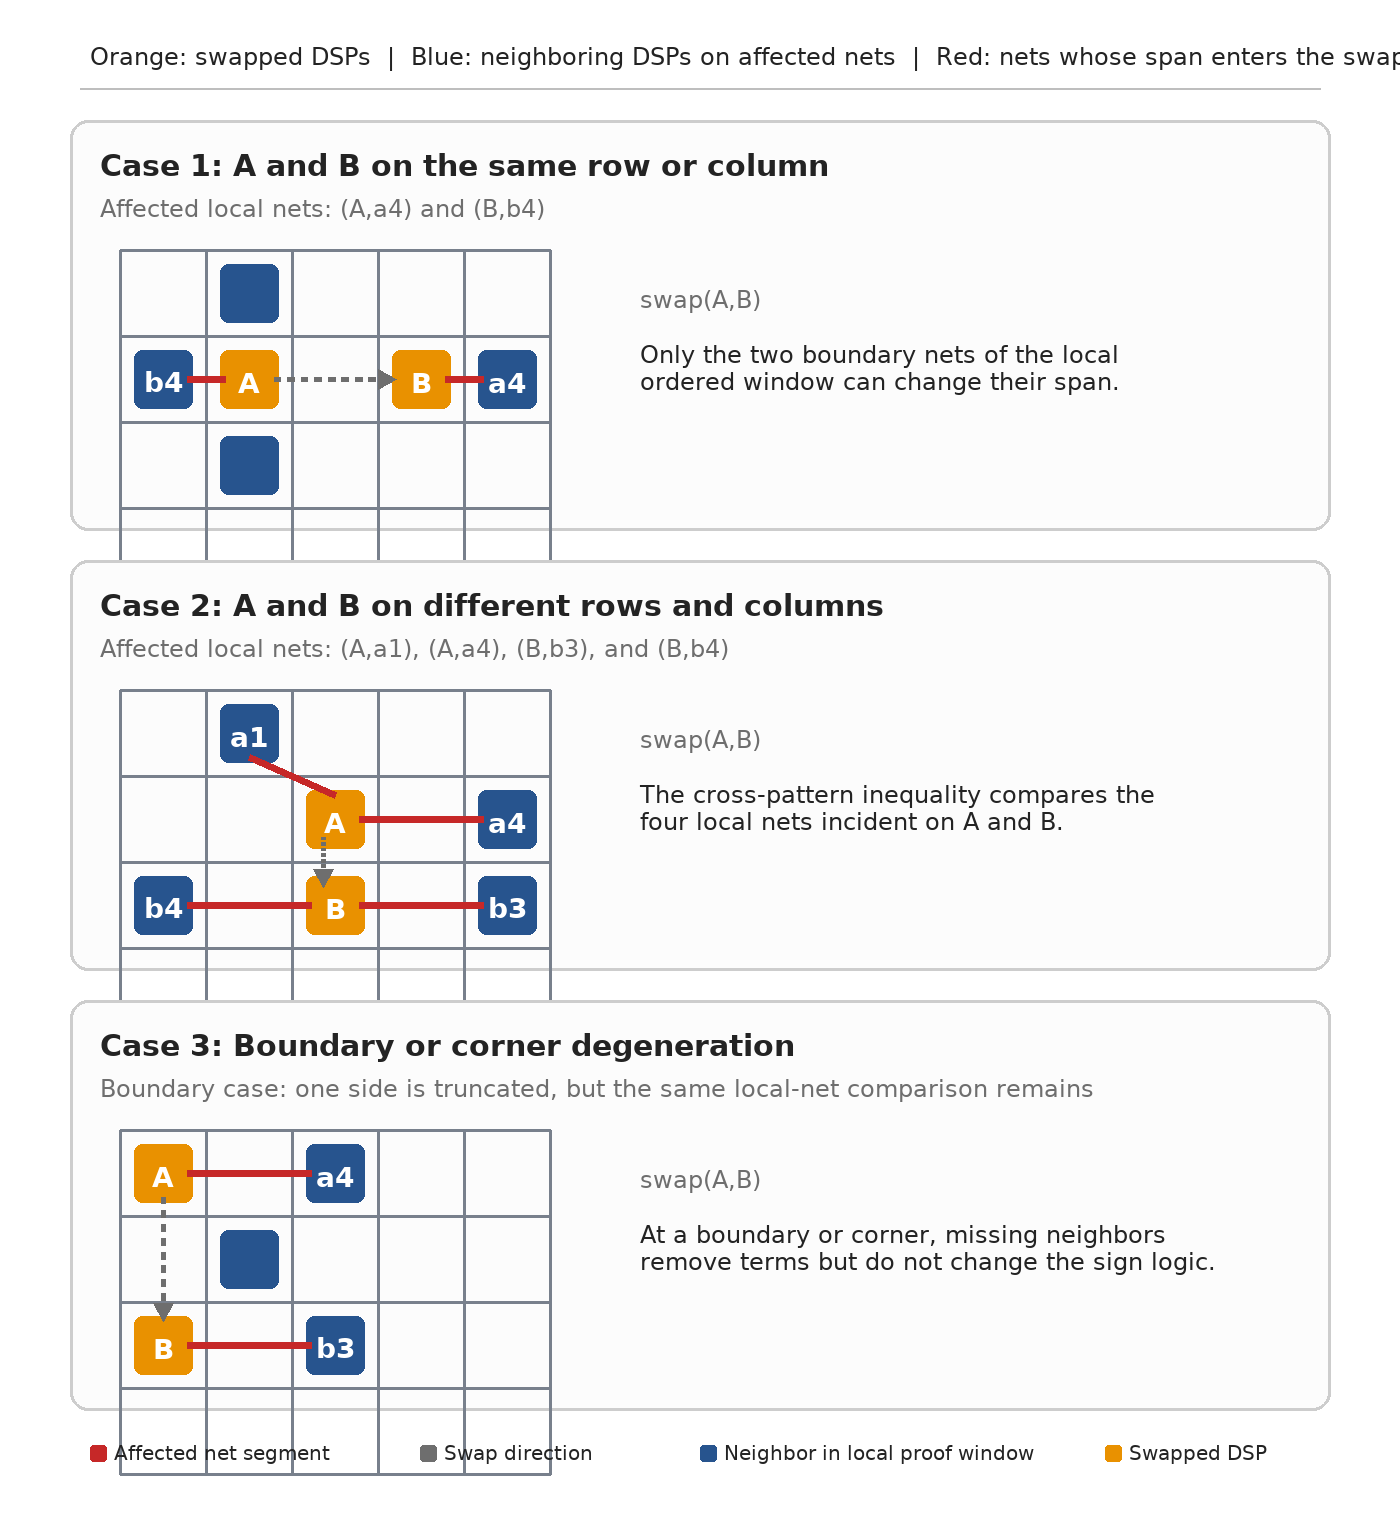
\includegraphics[width=0.98\columnwidth]{assets/oc_cases_precise.png}
\Description{Three local swap configurations used in the OC proof sketch. The first panel shows A and B on the same row or column, with affected local nets to neighboring macros. The second panel shows A and B on different rows and columns, with four affected local nets. The third panel shows a boundary or corner degeneration with truncated neighbors.}
\caption{Local swap patterns and affected nets in the OC proof sketch. The three panels correspond to the same-row or same-column case, the different-row and different-column case, and a boundary or corner degeneration. Red segments denote the local nets whose span enters the swap-local HPWL comparison, while blue blocks mark the neighboring DSPs referenced by the proof.}
\label{fig:oc_cases}
\end{figure}

For each pattern, the incident nets are partitioned into three groups: nets that are forced to become longer after the swap, nets whose contribution is unchanged, and nets that may become shorter. The key observation is that the forced increases always dominate the possible decreases, so the total HPWL change is nonnegative. Figure~\ref{fig:oc_cases} provides an intuitive view of the three local swap patterns. Two algebraic motifs summarize the calculation.

Let $Y(\cdot)$ denote the row or column coordinate used in the corresponding local comparison window. In other words, $Y(a)$, $Y(a_1)$, and related terms denote the ordered coordinate values that appear in the swap-local HPWL calculation for the pattern under discussion.

For the same-row or same-column pattern,
\begin{equation}
\Delta \mathrm{HPWL} = 2\bigl(Y(a4)-Y(b4)\bigr) \ge 0,
\label{eq:swap_same_line}
\end{equation}
where the neighboring terms appear in matched pairs and the swap can only preserve or increase the total span.

For the different-row/different-column pattern,
\begin{equation}
\Delta \mathrm{HPWL}
=
2\bigl(Y(a4)+Y(a1)-Y(b3)-Y(b4)\bigr) \ge 0.
\label{eq:swap_cross}
\end{equation}
This is the core cross-pattern inequality in the slide proof. Boundary and corner cases do not require separate principles; they reduce to the same two algebraic comparisons together with strictly positive contributions from nearby nets that are forced to lengthen after the swap.

Therefore, for any pair of DSP macros and for any swap distance, a two-swap applied to an OC-optimal solution cannot decrease HPWL. Proposition 1 follows.

This is the scientific role of \rsad in the present paper. OC is not introduced here as a heuristic convenience. Rather, it identifies a structured solution space that remains consistent with HPWL optimality in the single-column setting. Only after this justification do we impose OC and use it as the basis of the exact optimization framework below.

\subsection{From OC to an Ordered Objective}

After the above justification, we impose the order-consistency (OC) condition
\begin{equation}
y_{i,j} \le y_{i,j+1}, \qquad y_{i,j} \le y_{i+1,j},
\label{eq:oc}
\end{equation}
which is exactly the monotonicity structure introduced by \rsad.

Under OC, the relative order of every macro pair in a net is fixed. Therefore, each term $|y_{i_a,j_a}-y_{i_b,j_b}|$ in Eq.~(\ref{eq:weighted_hpwl}) has a determined sign and can be rewritten without the absolute value. Summing over all nets yields an ordered linear objective
\begin{equation}
\sum_{i,j} C_{i,j} y_{i,j},
\label{eq:ordered_linear}
\end{equation}
where $C_{i,j}$ aggregates the signed contributions of all incident nets to location $(i,j)$. This is the key algebraic step: once OC fixes pairwise ordering, the \hpwl objective is transformed from an unordered absolute-value objective into an ordered linear objective over placement labels.

\subsection{From Ordered Objective to State DAG}

Eq.~(\ref{eq:ordered_linear}) can be further rewritten into an incremental form indexed by placement order. For each location $(i,j)$, define
\begin{equation}
\phi_{i,j} = d_V \Bigl(
\underbrace{w^V_{i-1,j}}_{\text{up}}
\,+\,
\underbrace{w^H_{i,j-1}}_{\text{left}}
\,-\,
\underbrace{w^V_{i,j}}_{\text{down}}
\,-\,
\underbrace{w^H_{i,j}}_{\text{right}}
\Bigr),
\label{eq:phi}
\end{equation}
with out-of-range terms treated as zero. Here $\phi_{i,j}$ is the local coefficient of location $(i,j)$ in the ordered objective. If order label $\ell+1$ is assigned to location $(i,j)$, the incremental contribution is
\begin{equation}
c_{\ell}(i,j) = (\ell+1)\,\phi_{i,j}.
\label{eq:incremental_cost}
\end{equation}
Thus the total objective can be accumulated one placement step at a time.

We now define the state space. At level $\ell$, a state is
\begin{equation}
a = (a_1,\dots,a_m),
\end{equation}
where $a_i \in \{0,\dots,h\}$ is the number of already placed macros in row $i$, and $\ell=\sum_i a_i$ is the number of already assigned labels. Under OC, the frontier must remain monotone:
\begin{equation}
a_1 \ge a_2 \ge \cdots \ge a_m.
\label{eq:state_monotone}
\end{equation}
The source state is $(0,\dots,0)$ and the sink state is $(h,\dots,h)$.

\begin{figure}[t]
\centering
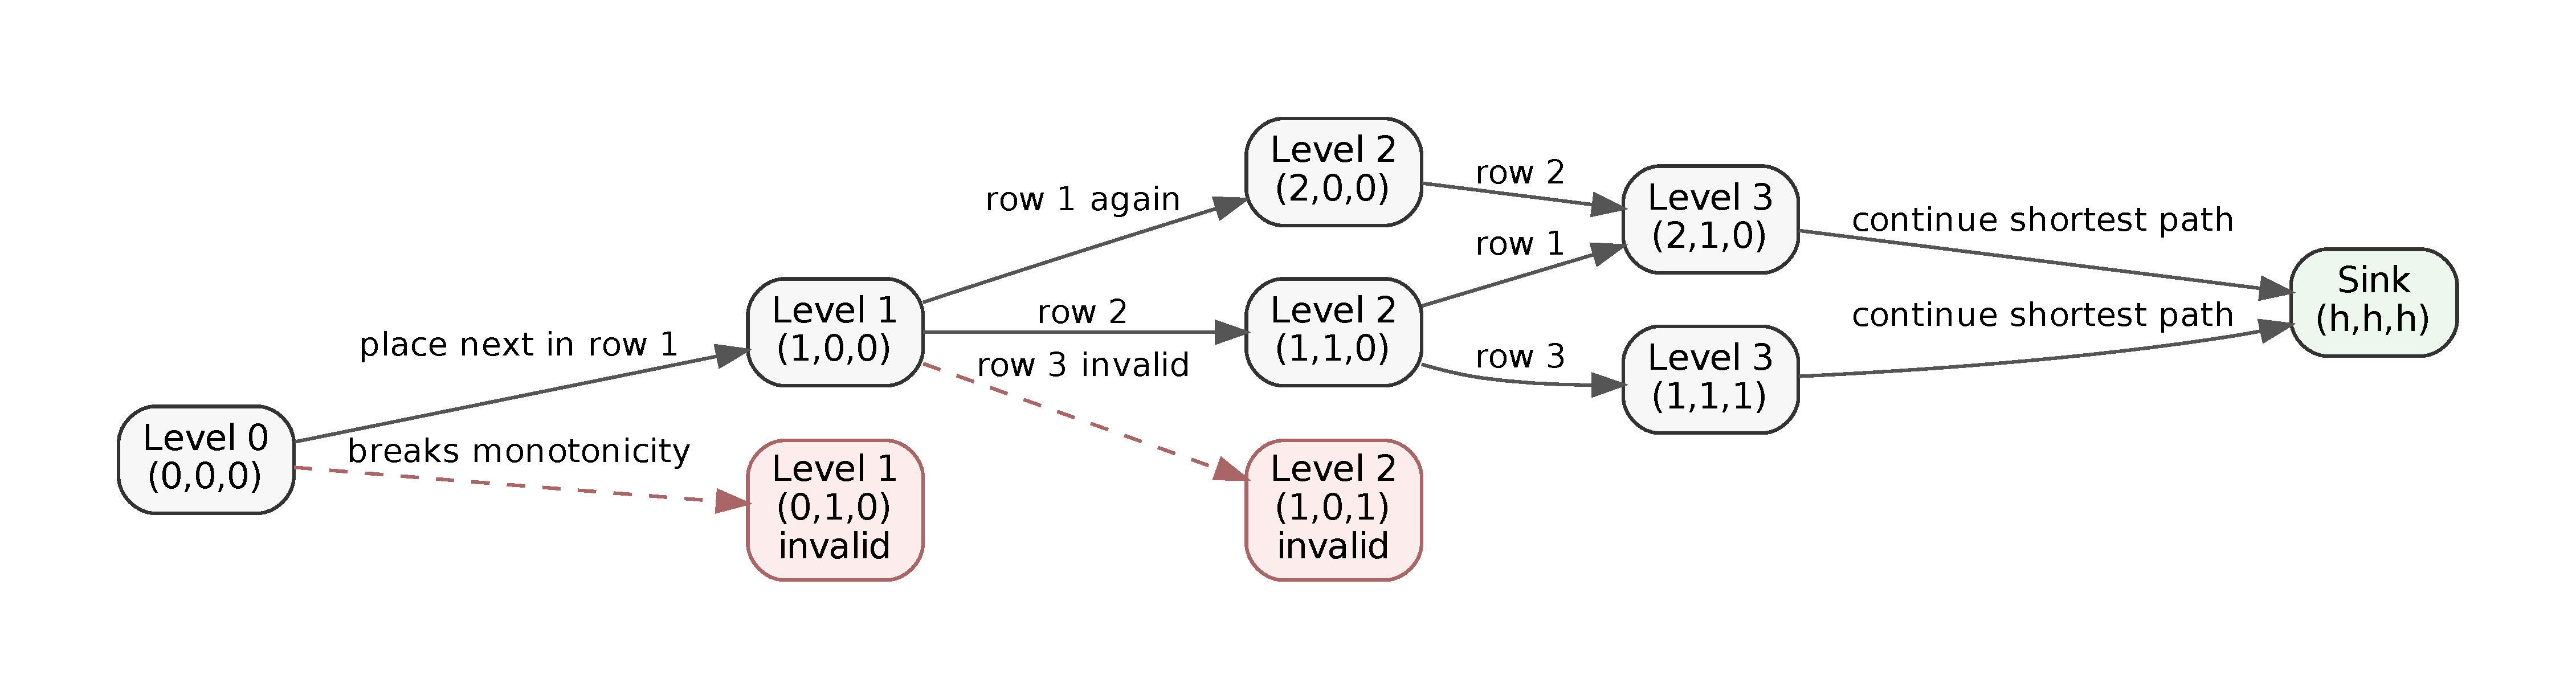
\includegraphics[width=0.95\columnwidth]{assets/state_dag_frontier.pdf}
\Description{A state-DAG illustration in which each node records how many positions have been filled in each row, and each valid edge increments one row count while preserving a monotone frontier.}
\caption{State-DAG view of the OC-constrained strip placement problem. A state records the monotone placement frontier, and each edge places exactly one new macro.}
\label{fig:state_dag}
\end{figure}

An edge in the DAG corresponds to incrementing exactly one row count. If state $a'$ is obtained from $a$ by increasing $a_i$ by one, then the next order label is assigned to location $(i,a_i+1)$. The move is legal only if the frontier remains monotone. Therefore each source-to-sink path corresponds to one feasible OC placement, and the path cost is the sum of all incremental costs. Let $\mathcal{P}(s,t)$ denote the set of all source-to-sink paths in the state DAG. The original optimization is reduced to
\begin{equation}
\min_{P \in \mathcal{P}(s,t)} \sum_{(a,a') \in P} c(a,a'),
\label{eq:dag_shortest_path}
\end{equation}
which is a shortest-path problem on a DAG.

\textbf{Key contribution.}
The main theoretical contribution of this paper is exactly this conversion from optimizing many weighted net HPWL terms to optimizing one shortest path on a state DAG.

\subsection{Dynamic Programming Solver}

Let $f_\ell(a)$ denote the minimum cost of reaching state $a$ after placing the first $\ell$ labels. Since the graph is acyclic, the DP recurrence is
\begin{equation}
f_{\ell+1}(a') = \min_{a \to a'} \bigl(f_\ell(a) + c(a,a')\bigr).
\label{eq:dp}
\end{equation}
The optimal placement is recovered by tracing the minimum-cost source-to-sink path. A forward-backward reconstruction scheme can be used to avoid storing the full DP table.

\subsection{CTR-Based Acceleration}

The exact DP solver is expensive on tall strips. A key acceleration is the central row-sweep (CTR) observation inherited from the \rsad line. When mapping an $m \times h$ array to one DSP column and $m > h > 6$, the middle part of the optimal placement exhibits a row-sweep pattern, called the CTR region in \rsad. What begins as an empirical observation can be converted into an algorithmic reduction.

Instead of solving the full $m \times h$ strip directly, we shrink it to an $h \times h$ core problem, solve that core exactly, and then expand the solution back to the original height. Concretely, the top and bottom bands are preserved from the solved square core, while the middle rows are filled by a row-sweep CTR band. In effect, an $m \times h$ mapping problem is converted into an $h \times h$ problem, and the resulting square solution is split into top and bottom parts with a row-sweep region inserted in the middle. This substantially reduces the computational burden while preserving the structural quality of the placement.

\subsection{Timing-Driven Weight Update}

The exact strip solver is placed inside an outer timing-driven loop. Starting from initial weights, the solver produces a weighted OC placement. That placement is then analyzed to obtain the longest edge, \wns, and \tns under the target $T$.

For each edge $e$, let $L_e$ denote its current geometric length. The slack-like quantity is
\begin{equation}
s_e = T - L_e.
\end{equation}
If all tracked edges satisfy $s_e \ge 0$, the current strip already satisfies the target. Otherwise, the most critical edges receive larger weights.

The weight update borrows the net-weight adaptation style used in DreamPlace 4.0~\cite{dreamplace4}. The solver keeps log-weights and momentum buffers:
\begin{equation}
\Delta \log w_e^{(t+1)} = \alpha\,\Delta \log w_e^{(t)} + \eta \log\bigl(1+c_e^{(t)}\bigr),
\label{eq:dreamplace_style_1}
\end{equation}
\begin{equation}
\log w_e^{(t+1)} = \log w_e^{(t)} + \Delta \log w_e^{(t+1)}.
\label{eq:dreamplace_style_2}
\end{equation}
Here $c_e^{(t)}$ is derived from the current violation magnitude, and only the most critical edges are strengthened in each round.

This creates a clean division of labor:
\begin{itemize}[leftmargin=*,topsep=2pt,itemsep=2pt]
\item the inner DP layer solves the weighted OC strip-placement problem exactly for fixed weights, and
\item the outer loop changes those weights to reduce the longest wires and improve timing.
\end{itemize}

This also explains the empirical tradeoff against \rsad. \rsad is highly effective when the objective is static HPWL minimization under OC. Our method keeps that OC structure and near-optimal HPWL behavior, but additionally drives down the longest wires, which yields better \wns and \fmax at the cost of only a very small HPWL increase.

\subsection{Discussion of Optimality Scope}

The exact optimality claim of this paper applies to the weighted state-DAG subproblem for a fixed set of net weights. The full timing-driven flow remains iterative because weights change between solves. Accordingly, the paper should claim:
\begin{itemize}[leftmargin=*,topsep=2pt,itemsep=2pt]
\item exact shortest-path optimality for the fixed-weight OC subproblem, and
\item empirical timing improvement for the full timing-driven outer loop.
\end{itemize}
